\documentclass[10pt]{scrartcl}

\usepackage[utf8]{inputenc}
\usepackage{tabularx}
\usepackage{longtable}
\usepackage[ngerman]{babel}
\usepackage[automark]{scrpage2}
\usepackage{amsmath,amssymb,amstext}
%\usepackage{mathtools}
\usepackage[]{color}
\usepackage[]{enumerate}
\usepackage{graphicx}
\usepackage{lastpage}
\usepackage[perpage,para,symbol*]{footmisc}
\usepackage{listings} 
\usepackage[pdfborder={0 0 0},colorlinks=false]{hyperref}
\usepackage[numbers,square]{natbib}
\usepackage{color}
\usepackage{colortbl}
\usepackage[absolute]{textpos}
\usepackage{float}
\usepackage{rotating}
\usepackage[colorinlistoftodos,textsize=small,textwidth=2cm,shadow,bordercolor=black,backgroundcolor={red!100!green!33},linecolor=black]{todonotes}

\lstset{numbers=left, numberstyle=\tiny, numbersep=5pt, breaklines=true, showstringspaces=false} 
\restylefloat{figure}

%changehere
\def\titletext{Praktikum 1}
\def\titletextshort{Praktikum 1}
\author{André Harms, Oliver Steenbuck}

\title{\titletext}

%changehere Datum der Übung
\date{15.11.2012}

\pagestyle{scrheadings}
%changehere
\ihead{UO, Gerken}
\ifoot{Generiert am:\\ \today}

\cfoot{Oliver Steenbuck, André Harms}


\ohead[]{\titletextshort}
\ofoot[]{{\thepage} / \pageref{LastPage}}

\setlength{\parindent}{0.0in}
\setlength{\parskip}{0.1in}

\begin{document}
\maketitle

\setcounter{tocdepth}{3}
\tableofcontents

\section{Verkäufer in Deutschland}
Die in Deutschland aktiven Verkäufe sind:
\begin{itemize}
	\item Helen Brolin
	\item Leif Shine
	\item Rob Carsson
	\item Tom Lindwall
\end{itemize}

\subsection{Warp AG}
Die Warp AG wird beliefert von:
\begin{itemize}
	\item Leif Shine
	\item Tom Lindwall
\end{itemize}

\section{Leif Shine}
In welchen Ländern ist Leif Shine aktiv ?
\begin{itemize}
	\item Deutschland
	\item Finnland
	\item Frankreich
	\item Mexico
	\item Polen
	\item Schweden
\end{itemize}


\section{Umsatzstärkste Firmen in Deutschland}
Die 10 Umsatzstärksten Firmen in Deutschland sind in dieser Reihenfolge:
\begin{enumerate}
	\item Grünewald
	\item Einracht GS
	\item Warp AG
	\item Boombastic
	\item Noch Einmal GMBH
	\item Gluderstedt
	\item Halle Köln
	\item Casual Clothing
	\item Autokleider
	\item Man Kleider
\end{enumerate}

\section{Drittbester Verkäufer}
Der drittbeste Verkäufer gemessen am Umsatz ist Frank Roll.

\section{Datenmodell}
Es soll hier kurz das in Abbildung \ref{pic:datenmodell} gezeigte Datenmodell erläutert werden:
Hier ist eine Struktur gewählt als derren zentrale Elemente die Tabellen \verb!Bestellungen' und \verb!Bestelldaten! die drei Komponenten 'Personal/Niederlassungen', 'Kunden/Märkte' und 'Produkte/Lieferanten' miteinander Verbinden.
Wobei hier auffällt, dass die automatisch importierte Tabelle \verb!Kontakte! an der Tabelle \verb!Bestellungen! angehängt ist, semantisch sinnvoller wäre es diese direkt an die Tabelle \verb!Kunden! anzuhängen.
 

\begin{figure}[H]
\begin{turn}{0}	
	\label{pic:datenmodell}
	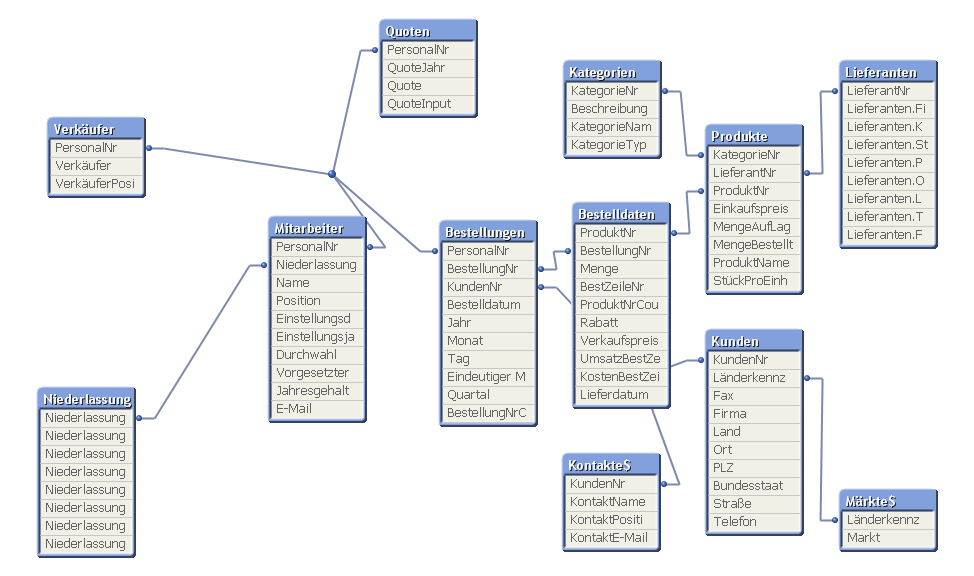
\includegraphics[scale=0.6]{export.png}
	\caption{Datenmodell Aufgabe 1} 
\end{turn}
\end{figure}

\end{document}

